This chapter describes a novel user interface paradigm for authoring mid-air gestures based on \emph{space discretization}, and its implementation as part of an end-to-end software tool designed to support end-users: \emph{Hotspotizer}. The design of the user interface paradigm

\section{Space Discretization}

Hotspotizer implements a paradigm based on space discretization for visualizing and manipulating gesture information. In the current implementation, we partition the space around the skeletal model tracked by the Kinect sensor into cubes that are 15cm on each side.

The total workspace is a large cube that is 3m on each side. While this is much larger than both the horizontal and vertical reach of many people; this is by design, to accommodates unusually tall users. The centroid of the cube that comprises the workspace is affixed to the "hip center" joint returned by the Kinect sensor. By specifying and tracking joint movements relative to the user’s skeletal model rather than the sensor’s position in real space, we aimed to leverage the user’s sense of proprioception \parencite{Shoemaker:2010} in gesturing.

To describe gestures, the cubic cells within the workspace may be marked to become hotspots – or \emph{hotspotized} – that register when a specified joint passes through them. Joints available for tracking are the hands, feet, elbows, knees and the head. Hotspotizing is accomplished by using front and side views in the Editor workspace. The front view is used to specify the horizontal and vertical positions of the hotspots. The side view is used to confirm the vertical and specify depth-wise positions. The design of this interaction style was inspired by architectural and engineering drawings.

In order to enable the authoring of dynamic movements along with static poses, we split movements into discrete keyframes. A timeline in the Editor module shows the keyframes and allows adding, removing, reordering and editing actions. Hotspots within subsequent frames do not need to be adjacent, but the frames need to be traversed in the correct order and within a certain time limit for a gesture to be recognized. The inter-frame timeout in Hotspotizer is 500ms. If more than 500ms elapses between a tracked limb engaging hotspots of subsequent frames, the gesture is not recognized.

Gestures designed using space discretization are dependent on location, scale and orientation with respect to the workspace, which is affixed to the user's hip or center of gravity. However, the paradigm affords a degree of spatial flexibility; hotspotizing a larger volume of cells allows for relaxed gesture boundaries.

This paradigm itself supports a versatile array of features. The size of hotspots could be made adjustable, even adaptive; to allow for fine gesturing close to the user’s body and more relaxed gesture boundaries at a distance. The total workspace volume could be made adjustable. The workspace could be defined in reference to limbs other than the center or in reference to the environment; supporting whole-body movements, a larger interaction space and rich proprioceptive interactions. The inter-frame timeout could be made adjustable to allow designs that exploit velocity and acceleration in gesturing. Hotspotizer does not implement these features. The design of the interface focuses on rapid development, simplification of expertise and lowering of skill barriers. Through pre-adjusted parameters for space discretization and timing, we reduce the complexity of the gesture authoring process and encapsulate the capabilities of the sensor. Future work may investigate empowering expert users with adjustability while maintaining the value added for non-experts.

% \subsection{Gesture Spotting in Discretized Space}

\section{Hotspotizer}
\label{sec:hotspotizer}

\begin{figure}[ht]
\centering
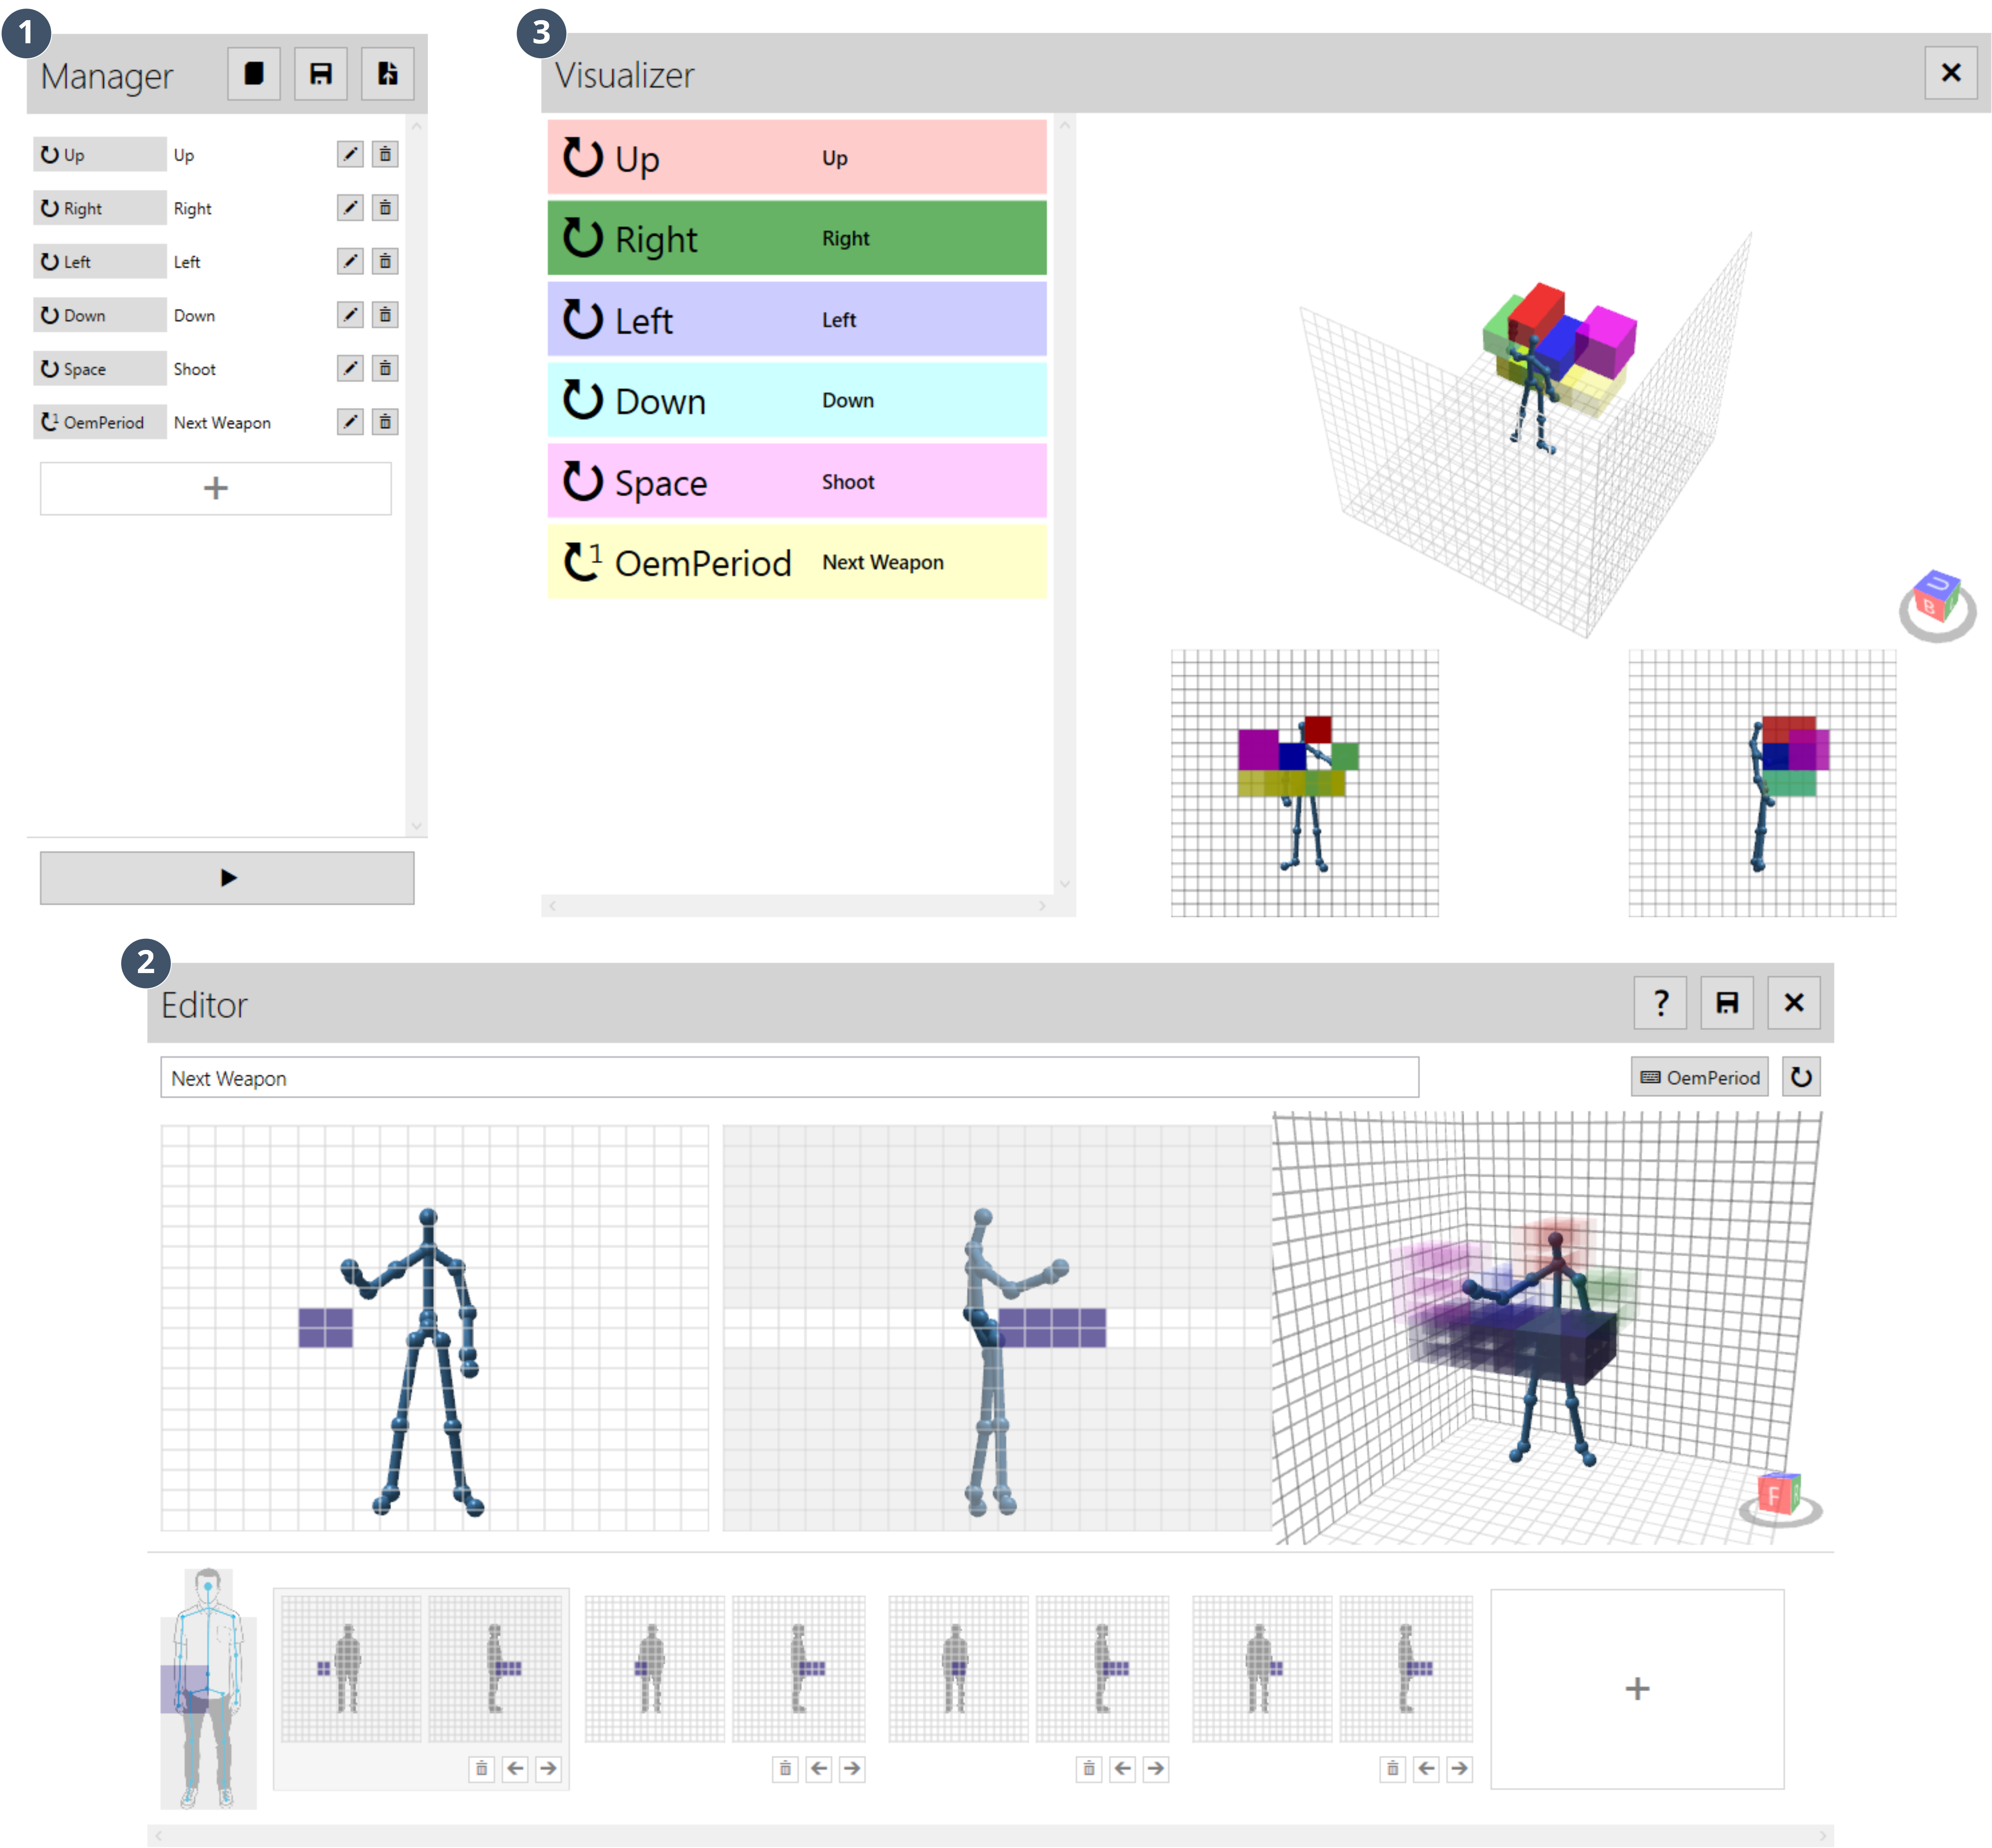
\includegraphics[width=\textwidth]{hotspotizer-modules}
\caption{Hotspotizer consists of three modules: (1) The Manager lists all of the gestures in the current collection and allows creating, saving and loading collections as well as adding, removing and editing individual gestures. (2) The Editor is the main workspace where gestures are authored. (3) The Visualizer provides interactive feedback on available and recognized gestures.}
\label{fig:hotspotizer-modules}
\end{figure}

\subsection{Usage}

To describe how mid-air gestures can be authored and mapped to keyboard events using Hotspotizer, lets consider the case of an end-user, Ali, who would like to adapt a document viewing application for gesture control. (Ali may require this functionality in contexts where touching a device to navigate a document is undesirable; e.g. when performing surgery on a patient or repairing an oily mechanism.) Figure~\ref{fig:workflow} depicts his workflow, and the numbers in parentheses throughout this section relate to the numbered panes in the figure.

\begin{figure}[ht]
\centering
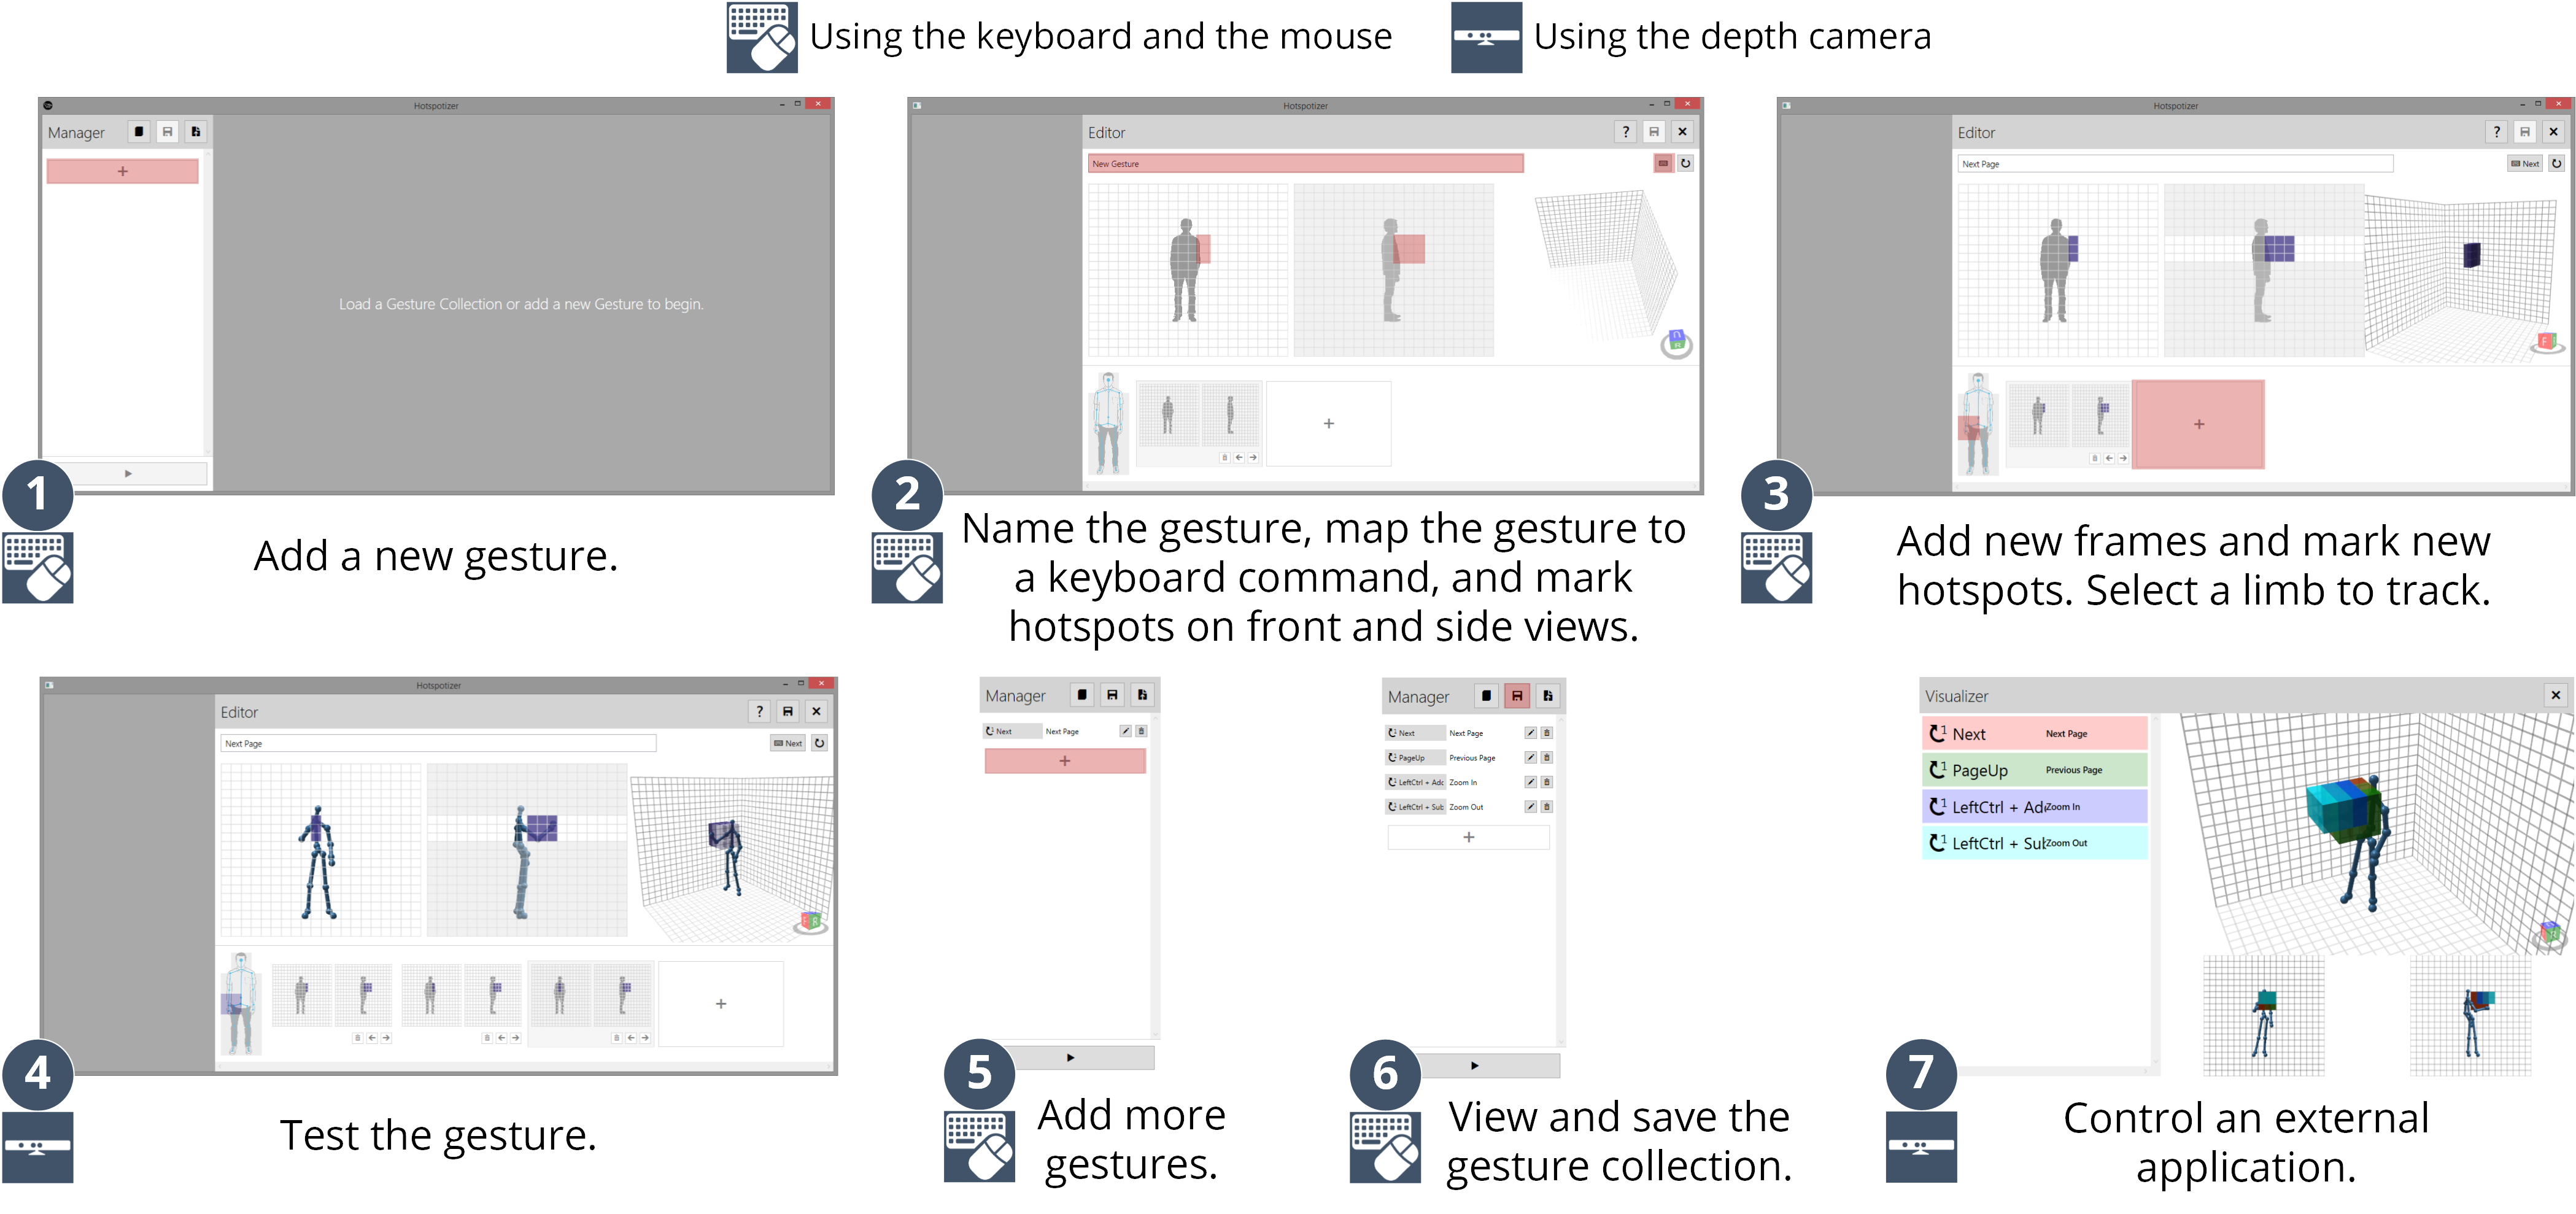
\includegraphics[width=\textwidth]{workflow}
\caption{The workflow of an end-user authoring gestures in Hotspotizer.}
\label{fig:workflow}
\end{figure}

Ali has to be able to cycle up and down between the pages of a document, as well as zoom in and out, using mid-air gestures. These actions may correspond to different keyboard commands depending on the document viewing application; lets assume that, respectively, the \emph{Page Up}, \emph{Page Down} keys and the \emph{Ctrl + Plus} and \emph{Ctrl + Minus} key combinations are used. To cycle between pages, the left hand is swiped in air as if turning the pages of a real, albeit large book. To zoom in and out, the right hand performs beckoning and pushing motions. Figure~\ref{fig:gestures} shows one way of describing these two gestures in terms of hotspots (for brevity, the \emph{page up} and \emph{zoom out} gestures are not shown).

\begin{SCfigure}[\sidecaptionrelwidth][ht]
\centering
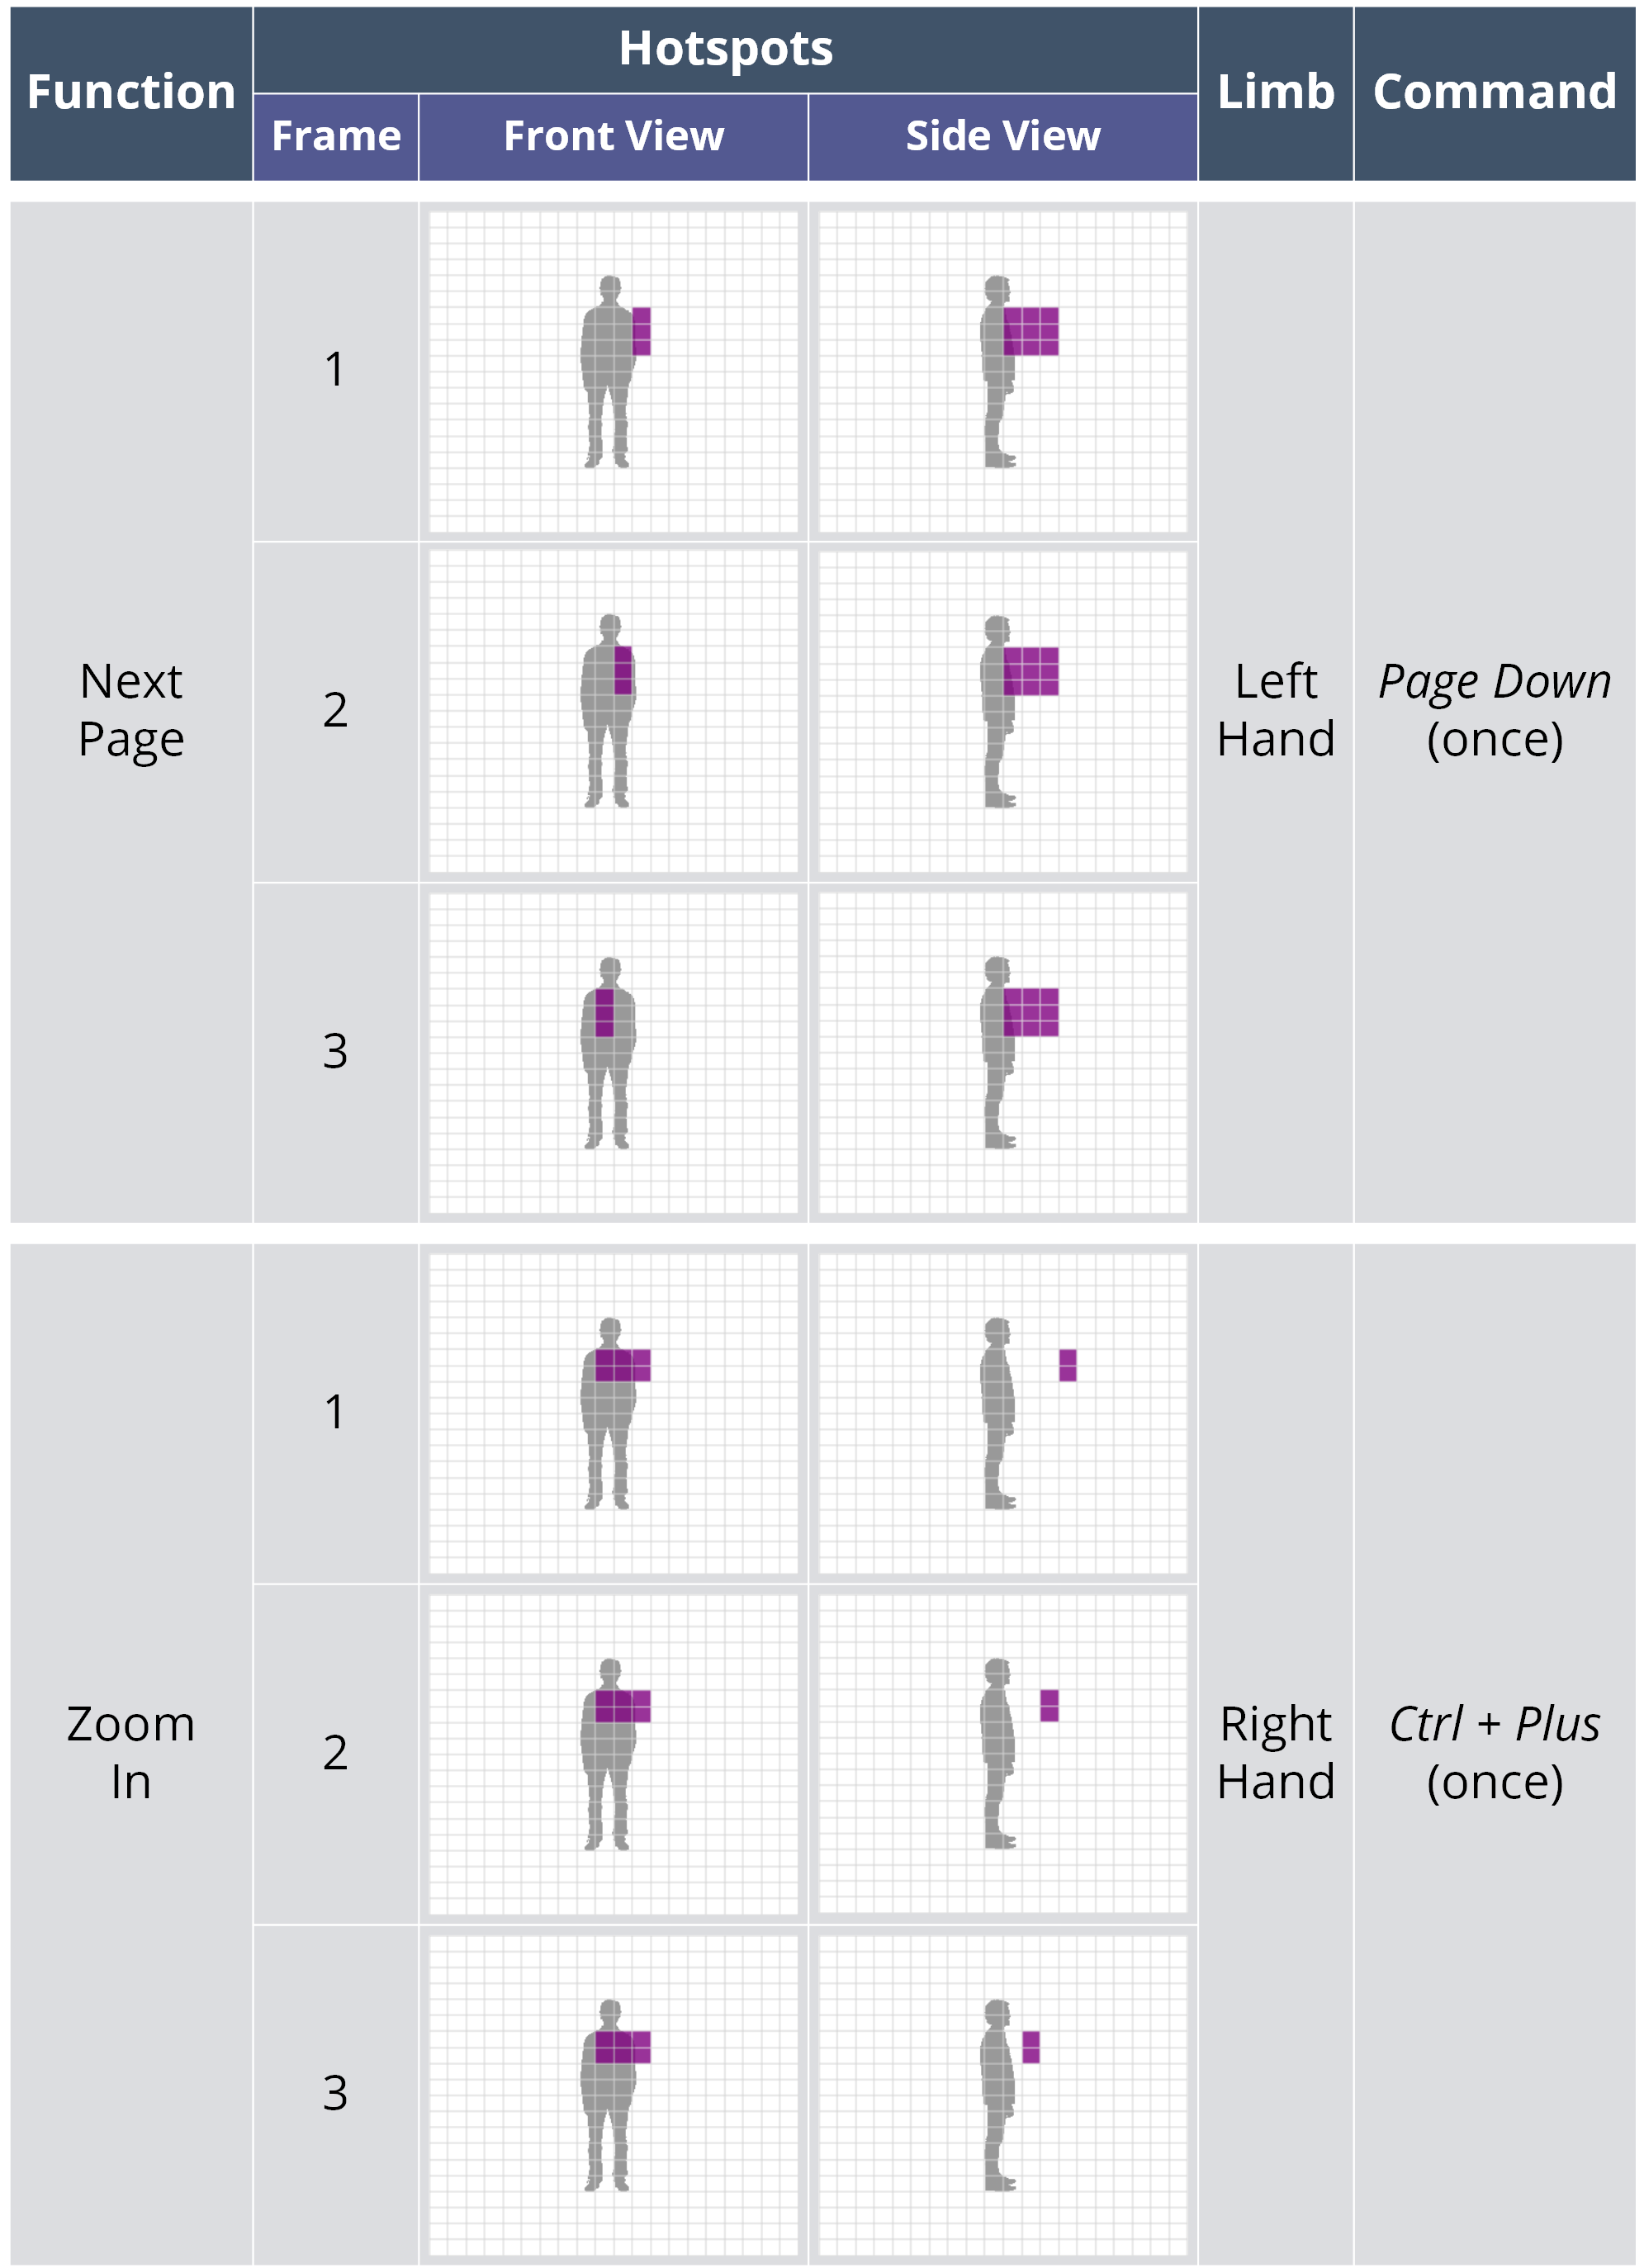
\includegraphics[width=.6\textwidth]{gestures}
\caption{\emph{Next page} and \emph{zoom in} gestures to control a document viewing application and the keyboard functionality that they map to. The diagrams show, respectively, hotspot arrangements for a swipe gesture and a beckoning motion.}
\label{fig:gestures}
\end{SCfigure}

\subsubsection{Creating and Editing Gestures}

Hotspotizer greets Ali with the Manager module containing empty gesture collection upon launch. Ali creates a new gesture in the collection, launching the Editor module \textbf{(1)}. Here, Ali assigns a name for the gesture for easy recall, specifies the Page Down key to be triggered when the gesture is performed, and confirms that the \emph{loop} toggle button is not checked – otherwise performing the gesture and holding the tracked limb over the hotspots in the last frame continues to hold down the keyboard key assigned to the gesture \textbf{(2)}.

Ali moves on to the main workspace where they use the front- and side-views over a representation of the tracked user to mark the positions of the hotspots for the first frame. Initially, all of the cells in the side view are disabled and grayed out. Marking cells on the front view enables the corresponding rows on the side view, whereupon Ali can mark the vertical and depth-wise position of their hotspots. Once hotspots are specified in all three dimensions by using these two grids, they appear on the 3D viewport on the right.

Once Ali completes marking the first frame’s hotspots, they can proceed to add another frame using the button next to the timeline of keyframes, and then another \textbf{(3)}. Finally, after marking the second and third frames’ hotspots, Ali selects the left hand as the limb that will be used in performing this gesture.

After saving the first gesture into the collection, Ali is taken back to the Manager module where they can add the remaining gestures and see the existing gestures to review, edit or delete them \textbf{(5)}. Once they are satisfied with the gesture collection they created, Ali can save the collection into a file for later use \textbf{(6)}.

\subsubsection{Testing Designs and Controlling External Applications}

At any time when using the Editor module, if they have a Kinect sensor connected to the computer, Ali may step in front of the sensor and see a rendering of the skeletal model of their body on the front, side and 3D viewports \textbf{(4)}. This feature can be used to rapidly test and tune hotspot locations at design time.

Testing over the whole gesture collection is available through the Visualizer module \textbf{(7)}. This module depicts a list of the gestures in the current collection and all of their hotspots on 3D, front and side viewports. Each gesture is shown in a different color. On the 3D viewport, transparency implies the order of hotspots. Hotspots glow when the tracked limb enters them in the correct order.

The Visualizer module also embeds the keyboard simulator. Launching the visualizer attaches a virtual keyboard to the system, which relays associated key events upon the successful performance of gestures. The visualization and the emulator continue to work when Hotspotizer is not in focus or is minimized.

\subsection{Implementation Details}

Hotspotizer was written in the \emph{C\#} programming language\footnote{\href{http://msdn.microsoft.com/en-us/library/kx37x362.aspx}{msdn.microsoft.com/library/kx37x362}}, using the \emph{Microsoft .NET Framework 4.5}\footnote{\href{http://www.microsoft.com/net}{microsoft.com/net}} and the \emph{Windows Presentation Foundation (WPF)}\footnote{\href{http://msdn.microsoft.com/en-us/library/ms754130.aspx}{msdn.microsoft.com/library/ms754130}} subsystem therein to create the user interface.

The following open source packages were used:

\begin{itemize}
\item \emph{Windows Input Simulator}\footnote{\href{http://inputsimulator.codeplex.com/}{inputsimulator.codeplex.com}} for keyboard emulation;
\item \emph{Json.NET}\footnote{\href{http://json.codeplex.com/}{json.codeplex.com}} for reading and writing gesture data to files; and,
\item \emph{Helix 3D Toolkit}\footnote{\href{http://helixtoolkit.codeplex.com/}{helixtoolkit.codeplex.com}} for 3D graphics.
\end{itemize}

Hotspotizer runs on Microsoft's \emph{Windows 7} and \emph{Windows 8} operating systems and requires the \emph{Microsoft Kinect Runtime}\footnote{\href{http://www.microsoft.com/en-us/download/details.aspx?id=40277}{microsoft.com/download/details.aspx?id=40277}}, and, if used with an \emph{Xbox Kinect} sensor, the \emph{Kinect SDK}\footnote{\href{http://www.microsoft.com/en-us/download/details.aspx?id=40278}{microsoft.com/download/details.aspx?id=40278}} to be installed on the user's computer.

We took care to make the process of installing and running Hotspotizer as straightforward as possible, in order to accommodate diverse user populations. We packaged it as a Windows application that can, as convention dictates, be installed from a single executable installer file, launched from the \emph{Start Menu}, and uninstalled from the operating system's \emph{Control Panel}. Upon launch, Hotspotizer checks for its external requirements, the Kinect Runtime and SDK. If the requirements are unavailable, it prompts the user to install them, providing links to the web pages where they can be downloaded (Figure~\ref{fig:warning-message}).

\begin{SCfigure}[3][ht]
\centering
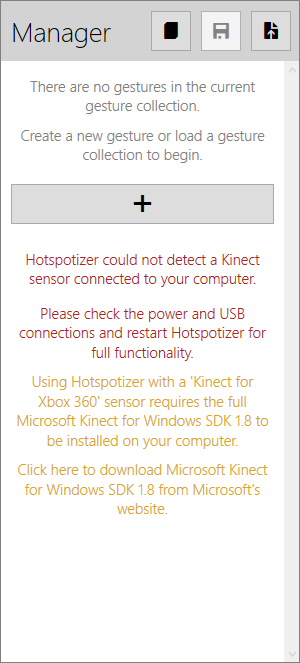
\includegraphics[width=.3\textwidth]{warning-message}
\caption{If the Kinect sensor is not functioning properly or if pre-requisite software is not installed on the computer, Hotspotizer prompts the user with a warning message.}
\label{fig:warning-message}
\end{SCfigure}

\subsection{Discussion}

The space discretization paradigm and its current implementation in Hotspotizer feature strengths and limitations that manifest as side effects of design choices.

One strength of the implementation is that gesture recognition is not influenced by the user's position and orientation within the sensor's field of view, provided that the depth image is not distorted and the sensor can build an accurate skeletal model of the user. Since the discretized workspace is affixed to the user's hip, hotspot locations are defined relative to the user's own body and the traversal of hotspots is detected properly as long as the skeletal model is built correctly. As a limitation of the depth sensor, skeletal modeling fails under certain conditions; e.g. the user turning their back to the sensor or engaging in contortions, the presence of objects that resemble a human form in the sensor's field of view, etc. Hotspotizer automatically hides the skeletal representation and halts gesture recognition when failures occur, and resumes operation when the sensor provides a skeletal model.

Certain limitations result from the design choice to prioritize leveraging a common infrastructure for end-users by mapping gestures to keyboard events. This obscures what \textcite{Hartmann:2007} call "association semantics" --- i.e. the relationship between commands relayed to applications from Hotspotizer and the resulting application behaviors --- and limits the expressive power of the gesture authoring paradigm.

A further limitation is that Hotspotizer currently does not support authoring continuous --- or \emph{online} \parencite{Hoste:2014} --- gestures that affect some variable while they are being performed (as opposed to \emph{offline} gestures that execute commands when the gesture is performed from the beginning to the end). This is not a limitation of the space discretization paradigm; since, theoretically, smaller portions of a gesture could be assigned to affect continuous variables (albeit in a quantized manner). Likewise, gestures that involve pointing at or manipulating dynamic user interface components in third party applications are not supported. This could be overcome by linking the discretized space model around the user with the virtual space of the user interface. However, these features require integration with a fully featured programming environment or language, which is beyond the design goals for this project. Exploring "tighter integration with application logic" \parencite{Hartmann:2007} to empower software developers is a goal for future work.
